\documentclass{beamer}
\usepackage[utf8]{inputenc}

\usetheme{Madrid}
\usecolortheme{default}
\usepackage{amsmath,amssymb,amsfonts,amsthm}
\usepackage{txfonts}
\usepackage{tkz-euclide}
\usepackage{listings}
\usepackage{adjustbox}
\usepackage{array}
\usepackage{tabularx}
\usepackage{gvv}
\usepackage{lmodern}
\usepackage{circuitikz}
\usepackage{tikz}
\usepackage{graphicx}

\setbeamertemplate{page number in head/foot}[totalframenumber]

\usepackage{tcolorbox}
\tcbuselibrary{minted,breakable,xparse,skins}



\definecolor{bg}{gray}{0.95}
\DeclareTCBListing{mintedbox}{O{}m!O{}}{%
	breakable=true,
	listing engine=minted,
	listing only,
	minted language=#2,
	minted style=default,
	minted options={%
		linenos,
		gobble=0,
		breaklines=true,
		breakafter=,,
		fontsize=\small,
		numbersep=8pt,
		#1},
	boxsep=0pt,
	left skip=0pt,
	right skip=0pt,
	left=25pt,
	right=0pt,
	top=3pt,
	bottom=3pt,
	arc=5pt,
	leftrule=0pt,
	rightrule=0pt,
	bottomrule=2pt,
	toprule=2pt,
	colback=bg,
	colframe=orange!70,
	enhanced,
	overlay={%
		\begin{tcbclipinterior}
			\fill[orange!20!white] (frame.south west) rectangle ([xshift=20pt]frame.north west);
	\end{tcbclipinterior}},
	#3,
}
\lstset{
	language=C,
	basicstyle=\ttfamily\small,
	keywordstyle=\color{blue},
	stringstyle=\color{orange},
	commentstyle=\color{green!60!black},
	numbers=left,
	numberstyle=\tiny\color{gray},
	breaklines=true,
	showstringspaces=false,
}
%------------------------------------------------------------
%This block of code defines the information to appear in the
%Title page
\title %optional
{4.13.41}
\date{}
%\subtitle{A short story}

\author % (optional)
{M Chanakya Srinivas- EE25BTECH11036}




\begin{document}


\frame{\titlepage}


\begin{frame}{Problem}
Find the area of the parallelogram formed by the lines
\[
y = m x, \quad y = m x + 1, \quad y = n x, \quad y = n x + 1.
\]
\end{frame}

%------------------------------------------
\begin{frame}{Normal Form of Lines}
The general equation of a line is
\begin{align}
\vec{n}^\top\vec{x} = c
\end{align}
where \(\vec{n}\) is the normal vector.

\begin{align}
y - m x &= 0 &\Rightarrow& \quad \vec{n}_1^\top\vec{x} = 0,\\
y - m x - 1 &= 0 &\Rightarrow& \quad \vec{n}_2^\top\vec{x} = 1,\\
y - n x &= 0 &\Rightarrow& \quad \vec{n}_3^\top\vec{x} = 0,\\
y - n x - 1 &= 0 &\Rightarrow& \quad \vec{n}_4^\top\vec{x} = 1.
\end{align}

\begin{align}
\vec{n}_1 = \vec{n}_2 = \myvec{-m \\ 1}, \quad 
\vec{n}_3 = \vec{n}_4 = \myvec{-n \\ 1}.
\end{align}
\end{frame}

%------------------------------------------
\begin{frame}{Intersection of Two Lines}
For two lines 
\(\vec{n}_1^\top\vec{x} = c_1\), 
\(\vec{n}_2^\top\vec{x} = c_2\),
\begin{align}
\myvec{\vec{n}_1^\top \\ \vec{n}_2^\top}\vec{x} = \myvec{c_1 \\ c_2}.
\end{align}
Hence,
\begin{align}
\vec{x} = 
\myvec{\vec{n}_1^\top \\ \vec{n}_2^\top}^{-1}\myvec{c_1 \\ c_2}.
\end{align}

\begin{align}
\vec{N} = \myvec{-m & 1 \\ -n & 1}, \quad
\vec{N}^{-1} = \frac{1}{n - m}\myvec{1 & -1 \\ n & -m}.
\end{align}
\end{frame}

%------------------------------------------
\begin{frame}{Vertices of Parallelogram}
\begin{align}
\vec{A} &= \vec{N}^{-1}\myvec{0 \\ 0} 
= \myvec{0 \\ 0},\\[4pt]
\vec{B} &= \vec{N}^{-1}\myvec{1 \\ 0} 
= \frac{1}{n-m}\myvec{1 \\ n},\\[4pt]
\vec{C} &= \vec{N}^{-1}\myvec{1 \\ 1} 
= \myvec{0 \\ 1},\\[4pt]
\vec{D} &= \vec{N}^{-1}\myvec{0 \\ 1} 
= \frac{1}{n-m}\myvec{-1 \\ -m}.
\end{align}

Thus,
\begin{align}
\vec{A} = \myvec{0 \\ 0}, \quad
\vec{B} = \frac{1}{n-m}\myvec{1 \\ n}, \quad
\vec{C} = \myvec{0 \\ 1}, \quad
\vec{D} = \frac{1}{n-m}\myvec{-1 \\ -m}.
\end{align}
\end{frame}

%------------------------------------------
\begin{frame}{Area of Parallelogram}
Two adjacent sides:
\begin{align}
\vec{B}-\vec{A} &= \frac{1}{n-m}\myvec{1 \\ n},\\
\vec{D}-\vec{A} &= \frac{1}{n-m}\myvec{-1 \\ -m}.
\end{align}

Area:
\begin{align}
\text{Area} 
&= \abs{(\vec{B}-\vec{A}) \times (\vec{D}-\vec{A})} \\
&= \left|\frac{1}{(n-m)^2}
\det\myvec{1 & -1 \\ n & -m}\right|\\
&= \frac{1}{|m - n|}.
\end{align}
\end{frame}
\begin{frame}{FINAL ANSWER}
    \[
\boxed{\text{Area of the parallelogram} = \frac{1}{|m - n|}}
\]
\end{frame}


  \begin{frame}[fragile]{C code}
\begin{lstlisting}

#include <math.h>

// Make the symbol visible in the shared object
__attribute__((visibility("default")))
double parallelogram_area(double x1, double y1, double x2, double y2) {
    // Cross product magnitude
    return fabs(x1 * y2 - x2 * y1);
}

 \end{lstlisting}
\end{frame}
\begin{frame}[fragile]{Python code through shared output}
\begin{lstlisting}
 import ctypes
import numpy as np
import matplotlib.pyplot as plt

# Load the compiled shared library
lib = ctypes.CDLL('./libpara.so')
lib.parallelogram_area.argtypes = [ctypes.c_double, ctypes.c_double, ctypes.c_double, ctypes.c_double]
lib.parallelogram_area.restype = ctypes.c_double

# Slopes
m = 1
n = -1
 \end{lstlisting}
\end{frame}
\begin{frame}[fragile]{Python code through shared output}
\begin{lstlisting}

# Function to get intersection of two lines: y = m1 x + c1 and y = m2 x + c2
def line_intersection(m1, c1, m2, c2):
    x = (c2 - c1) / (m1 - m2)
    y = m1 * x + c1
    return x, y

# Calculate all four vertices (intersections)
P1 = line_intersection(m, 0, n, 0)       # y=mx and y=nx
P2 = line_intersection(m, 0, n, 1)       # y=mx and y=nx+1
P3 = line_intersection(m, 1, n, 1)       # y=mx+1 and y=nx+1
P4 = line_intersection(m, 1, n, 0)       # y=mx+1 and y=nx

# Convert to numpy arrays for vector operations
P1 = np.array(P1)
P2 = np.array(P2)
 \end{lstlisting}
\end{frame}
\begin{frame}[fragile]{Python code through shared output}
\begin{lstlisting}

P3 = np.array(P3)
P4 = np.array(P4)

# Compute side vectors for area calculation (two adjacent sides from P1)
vec1 = P2 - P1
vec2 = P4 - P1

# Call the C function for area
area = lib.parallelogram_area(vec1[0], vec1[1], vec2[0], vec2[1])

# ----- Plotting Section -----

# X range for lines plotting
x_vals = np.linspace(-2, 2, 400)
 \end{lstlisting}
\end{frame}
\begin{frame}[fragile]{Python code through shared output}
\begin{lstlisting}

# Lines y = mx and y = mx + 1
y_m = m * x_vals
y_m1 = m * x_vals + 1

# Lines y = nx and y = nx + 1
y_n = n * x_vals
y_n1 = n * x_vals + 1

plt.figure(figsize=(8, 8))
plt.plot(x_vals, y_m, label=r'$y = mx$', color='blue')
plt.plot(x_vals, y_m1, label=r'$y = mx + 1$', linestyle='--', color='blue')
plt.plot(x_vals, y_n, label=r'$y = nx$', color='red')
plt.plot(x_vals, y_n1, label=r'$y = nx + 1$', linestyle='--', color='red')
 \end{lstlisting}
\end{frame}
\begin{frame}[fragile]{Python code through shared output}
\begin{lstlisting}

# Parallelogram vertices for plotting (close the polygon by adding P1 again)
vertices_x = [P1[0], P2[0], P3[0], P4[0], P1[0]]
vertices_y = [P1[1], P2[1], P3[1], P4[1], P1[1]]

# Plot parallelogram
plt.plot(vertices_x, vertices_y, 'k-', linewidth=2, label='Parallelogram')
plt.fill(vertices_x, vertices_y, color='gray', alpha=0.3)

# Label vertices
for i, (xv, yv) in enumerate(zip(vertices_x[:-1], vertices_y[:-1]), 1):
    plt.text(xv, yv, f'P{i}', fontsize=12, ha='right', va='bottom')
 \end{lstlisting}
\end{frame}
\begin{frame}[fragile]{Python code through shared output}
\begin{lstlisting}

# Show area on plot
plt.text(-1.5, 1.5, f'Area = {area:.4f}', fontsize=14, color='green',
         bbox=dict(facecolor='white', alpha=0.8))

# Axis formatting
plt.axhline(0, color='black', linewidth=0.5)
plt.axvline(0, color='black', linewidth=0.5)
 \end{lstlisting}
\end{frame}
\begin{frame}[fragile]{Python code through shared output}
\begin{lstlisting}

plt.grid(True, linestyle='--', alpha=0.5)
plt.legend()
plt.title('Parallelogram formed by lines $y=mx$, $y=mx+1$, $y=nx$, $y=nx+1$\n(Area via C shared library)')
plt.xlabel('x-axis')
plt.ylabel('y-axis')
plt.axis('equal')
plt.xlim(-2, 2)
plt.ylim(-2, 2)

plt.show()

 \end{lstlisting}
 \end{frame}

\begin{frame}[fragile]{Only Python code}
\begin{lstlisting}
import numpy as np
import matplotlib.pyplot as plt

def line_intersect(n1, c1, n2, c2):
    """
    Find intersection point of two lines:
    n1.T * x = c1
    n2.T * x = c2
    Inputs:
        n1, n2: (2,) or (2,1) normal vectors to lines
        c1, c2: scalars
    Returns:
        p: (2,1) intersection point
    """
    N = np.column_stack((n1.flatten(), n2.flatten()))  # 2x2 matrix
    C = np.array([c1, c2])
    p = np.linalg.solve(N, C)
    return p.reshape(2,1)
 \end{lstlisting}
 \end{frame}

\begin{frame}[fragile]{Only Python code}
\begin{lstlisting}
def line_dir_pt(direction, point, k1, k2, num=100):
    """
    Generate points on a line given direction and a point.
    direction: (2,) array
    point: (2,) array
    k1, k2: scalar parameters along the line
    num: number of points
    Returns: 2 x num array of points
    """
    k = np.linspace(k1, k2, num)
    line_pts = point.reshape(2,1) + direction.reshape(2,1) * k
    return line_pts

# Slopes
m = 1
n = -1
 \end{lstlisting}
 \end{frame}

\begin{frame}[fragile]{Only Python code}
\begin{lstlisting}
# Normals (for line: y = m x + c  => -m x + y = c)
n1 = np.array([-m, 1])
n2 = np.array([-m, 1])
n3 = np.array([-n, 1])
n4 = np.array([-n, 1])

# Constants c
c1 = 0
c2 = 1
c3 = 0
c4 = 1

# Find intersection points
P1 = line_intersect(n1, c1, n3, c3)
P2 = line_intersect(n1, c1, n4, c4)
P3 = line_intersect(n2, c2, n4, c4)
P4 = line_intersect(n2, c2, n3, c3)

# Parallelogram points array
parallelogram = np.hstack((P1, P2, P3, P4, P1))
 \end{lstlisting}
 \end{frame}

\begin{frame}[fragile]{Only Python code}
\begin{lstlisting}
# Calculate area via cross product
vec1 = P2 - P1
vec2 = P4 - P1
area = abs(np.cross(vec1.flatten(), vec2.flatten()))

# Direction vectors for lines (x direction)
dir_m = np.array([1, m])
dir_n = np.array([1, n])

# Generate line points for plotting
k1, k2 = -5, 5

line_m0 = line_dir_pt(dir_m, np.array([0,0]), k1, k2)
line_m1 = line_dir_pt(dir_m, np.array([0,1]), k1, k2)
line_n0 = line_dir_pt(dir_n, np.array([0,0]), k1, k2)
line_n1 = line_dir_pt(dir_n, np.array([0,1]), k1, k2)
 \end{lstlisting}
 \end{frame}

\begin{frame}[fragile]{Only Python code}
\begin{lstlisting}
# Plotting
plt.figure(figsize=(8,8))
plt.plot(line_m0[0], line_m0[1], label='y = m x', color='blue')
plt.plot(line_m1[0], line_m1[1], label='y = m x + 1', linestyle='--', color='blue')
plt.plot(line_n0[0], line_n0[1], label='y = n x', color='red')
plt.plot(line_n1[0], line_n1[1], label='y = n x + 1', linestyle='--', color='red')

plt.plot(parallelogram[0], parallelogram[1], 'k-', linewidth=2, label='Parallelogram')
plt.fill(parallelogram[0], parallelogram[1], 'grey', alpha=0.3)

for i, P in enumerate([P1, P2, P3, P4], 1):
    plt.plot(P[0], P[1], 'ko')
    plt.text(P[0] + 0.1, P[1] + 0.1, f'P{i}', fontsize=12)
 \end{lstlisting}
 \end{frame}

\begin{frame}[fragile]{Only Python code}
\begin{lstlisting}
plt.text(-4.5, 4, f'Area = {area:.3f}', fontsize=14, color='green',
         bbox=dict(facecolor='white', alpha=0.8))

plt.axhline(0, color='black', lw=0.5)
plt.axvline(0, color='black', lw=0.5)
plt.grid(True, linestyle='--', alpha=0.6)
plt.axis('equal')
 \end{lstlisting}
 \end{frame}

\begin{frame}[fragile]{Only Python code}
\begin{lstlisting}
plt.xlim(-5, 5)
plt.ylim(-5, 5)
plt.xlabel('x-axis')
plt.ylabel('y-axis')
plt.title('Parallelogram formed by lines y=mx, y=mx+1, y=nx, y=nx+1')
plt.legend()
plt.show()


  \end{lstlisting}
\end{frame}
\begin{frame}{PLOTS}
    \begin{figure}
        \centering
        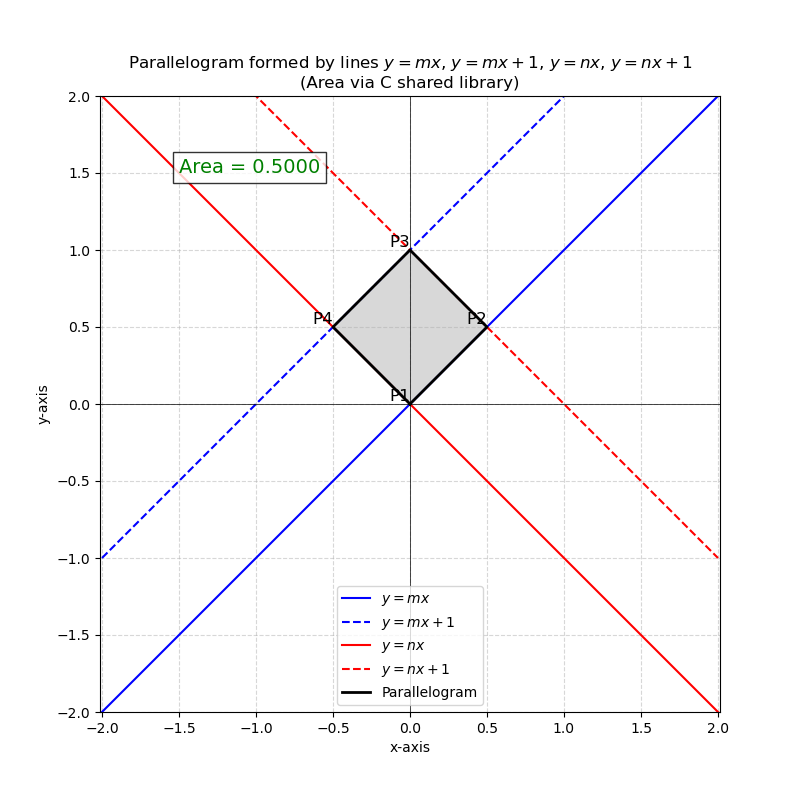
\includegraphics[width=0.9\columnwidth]{figs/Figure_81.png}
        \caption{}
        \label{fig:placeholder}
    \end{figure}
\end{frame}
\begin{frame}{PLOTS}
    \begin{figure}
        \centering
        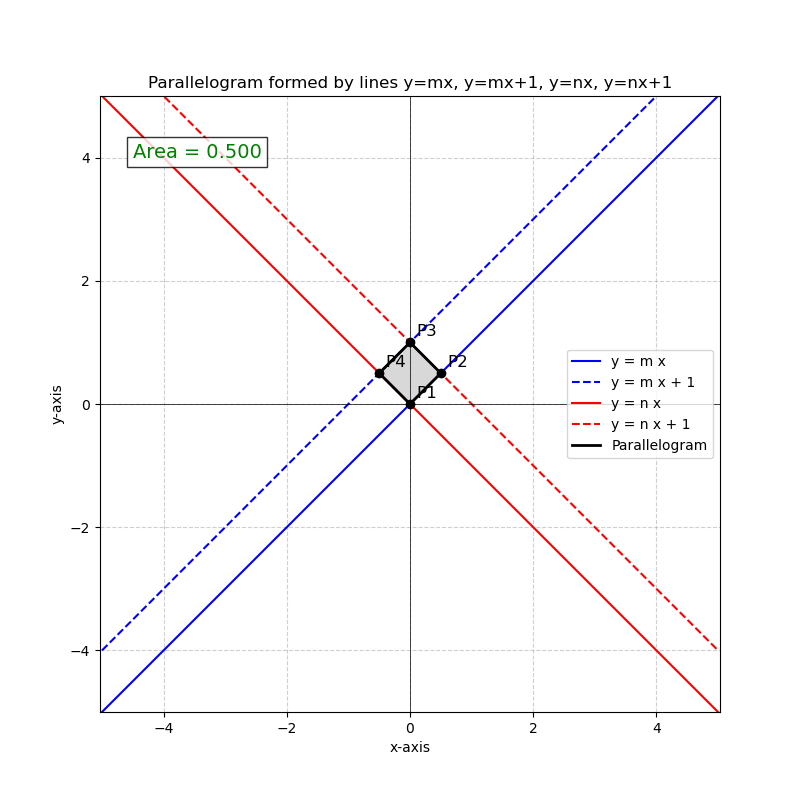
\includegraphics[width=0.9\columnwidth]{figs/fig82.png}
        \caption{}
        \label{fig:placeholder}
    \end{figure}
\end{frame}
\end{document}
